% allgem. Dokumentenformat
\documentclass[a4paper,12pt,headsepline]{scrartcl}

% weitere Pakete
% Grafiken aus PNG Dateien einbinden
\usepackage{graphicx}

%for psuedo code
\usepackage[linesnumbered, ruled]{algorithm2e} 
%
\newcommand{\nosemic}{\SetEndCharOfAlgoLine{\relax}}% Drop semi-colon ;
\newcommand{\dosemic}{\SetEndCharOfAlgoLine{\string;}}% Reinstate
\newcommand{\pushline}{\Indp}% Indent
\newcommand{\popline}{\Indm\dosemic}% Undent
%\stackMath
%\[\def\stacktype{L}\setstackgap{L}{.4ex}
%x\mathrel{\stackon{\cup}{\scriptscriptstyle+}}y
%\mathrel{\stackon{\cup}{\scriptscriptstyle-}}z
%\]
%
% Incompatibility with ctable, both implement package transparency
% http://tex.stackexchange.com/questions/253401/tikz-and-ctable-incompatibility-gives-error-when-printing
\usepackage{tikz}
\usetikzlibrary{calc, shapes, arrows}
% \circled is used for circling chars
\newcommand*\circled[1]{\tikz[baseline=(char.base)]{\node[shape=circle,draw,inner sep=2pt] (char) {#1};}}

% Eurozeichen einbinden
\usepackage[right]{eurosym}

% Incompatibility tikz, both implement package transparency
%\usepackage{ctable}

% Umlaute unter UTF8 nutzen
\usepackage[utf8]{inputenc}

% Zeichenencoding
\usepackage[T1]{fontenc}

\usepackage{lmodern}
\usepackage{fix-cm}

\usepackage{svg}

% floatende Bilder ermöglichen
%\usepackage{floatflt}

% mehrseitige Tabellen ermöglichen
\usepackage{longtable}

\usepackage{afterpage}

% Unterstützung für Schriftarten
%\newcommand{\changefont}[3]{ 
%\fontfamily{#1} \fontseries{#2} \fontshape{#3} \selectfont}

\setcounter{secnumdepth}{4}
\setcounter{tocdepth}{4}

% Packet für Seitenrandabständex und Einstellung für Seitenränder
\usepackage{geometry}
\geometry{left=3.5cm, right=2cm, top=2.5cm, bottom=2cm}

% Paket für Boxen im Text
\usepackage{fancybox}

% bricht lange URLs "schoen" um
\usepackage[hyphens,obeyspaces,spaces]{url}

% Paket für Textfarben
\usepackage{color}

% Mathematische Symbole importieren
\usepackage{amssymb}

% Writing text over arrows
\usepackage{mathtools}

% auf jeder Seite eine Überschrift (alt, zentriert)
%\pagestyle{headings}

% neue Kopfzeilen mit fancypaket
\usepackage{fancyhdr} %Paket laden
\pagestyle{fancy} %eigener Seitenstil
\fancyhf{} %alle Kopf- und Fußzeilenfelder bereinigen
\fancyhead[L]{\nouppercase{\leftmark}} %Kopfzeile links
\fancyhead[C]{} %zentrierte Kopfzeile
\fancyhead[R]{\thepage} %Kopfzeile rechts
\renewcommand{\headrulewidth}{0.4pt} %obere Trennlinie
%\fancyfoot[C]{\thepage} %Seitennummer
%\renewcommand{\footrulewidth}{0.4pt} %untere Trennlinie

% für Tabellen
\usepackage{array}

% Runde Klammern für Zitate
%\usepackage[numbers,round]{natbib}

% Festlegung Art der Zitierung - Havardmethode: Abkuerzung Autor + Jahr
\bibliographystyle{alphadin}

% Schaltet den zusätzlichen Zwischenraum ab, den LaTeX normalerweise nach einem Satzzeichen einfügt.
\frenchspacing

% Paket für Zeilenabstand
\usepackage{setspace}

% für Bildbezeichner
\usepackage{capt-of}

% für Stichwortverzeichnis
\usepackage{makeidx}

% für Listings
\usepackage{listings}
\lstset{numbers=left, numberstyle=\tiny, numbersep=5pt, keywordstyle=\color{black}\bfseries, stringstyle=\ttfamily,showstringspaces=false,basicstyle=\footnotesize,captionpos=b}
\lstset{language=java}

% Indexerstellung
\makeindex

% Abkürzungsverzeichnis
\usepackage[english]{nomencl}
\let\abbrev\nomenclature

% Abkürzungsverzeichnis LiveTex Version
\renewcommand{\nomname}{Abbreviations}
\setlength{\nomlabelwidth}{.25\hsize}
\renewcommand{\nomlabel}[1]{#1 \dotfill}
\setlength{\nomitemsep}{-\parsep}
\makenomenclature
%\makeglossary

% Abkürzungsverzeichnis TeTEX Version
% \usepackage[german]{nomencl}
% \makenomenclature
% %\makeglossary
% \renewcommand{\nomname}{Abkürzungsverzeichnis}
% \setlength{\nomlabelwidth}{.25\hsize}
% \renewcommand{\nomlabel}[1]{#1 \dotfill}
% \setlength{\nomitemsep}{-\parsep}

% Disable single lines at the start of a paragraph (Schusterjungen)
\clubpenalty = 10000
% Disable single lines at the end of a paragraph (Hurenkinder)
\widowpenalty = 10000
\displaywidowpenalty = 10000

\begin{document}
\begin{center}
\resizebox{\linewidth}{!}{
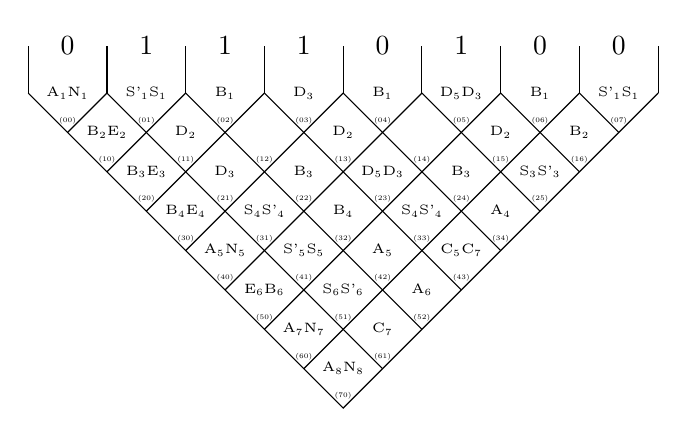
\begin{tikzpicture}[baseline]
\newcommand{\myfontvars}[1]{
\fontsize{4.9}{12}\selectfont{#1}
}\newcommand{\myfontnumbering}[1]{
\fontsize{2.5}{12}\selectfont{#1}
}%Outer hull
%Tip of the pyramidLatex
\coordinate (tip) at (4,-4);
\foreach \i in {0,...,8} {
 	\coordinate (\i) at (\i,0);
}
%Draw the left and right line of the pyramidLatex pointing downwards
\draw (0) -- (tip) -- (8);
%Grid lines direction down-left to top-right
\coordinate (dl1) at (0.5,-0.5);
\coordinate (dl2) at (1.0,-1.0);
\coordinate (dl3) at (1.5,-1.5);
\coordinate (dl4) at (2.0,-2.0);
\coordinate (dl5) at (2.5,-2.5);
\coordinate (dl6) at (3.0,-3.0);
\coordinate (dl7) at (3.5,-3.5);
\draw (dl1) -- (1,0);
\draw (dl2) -- (2,0);
\draw (dl3) -- (3,0);
\draw (dl4) -- (4,0);
\draw (dl5) -- (5,0);
\draw (dl6) -- (6,0);
\draw (dl7) -- (7,0);
%Grid lines direction down-right to top-left
\coordinate (dr1) at (4.5,-3.5);
\coordinate (dr2) at (5.0,-3.0);
\coordinate (dr3) at (5.5,-2.5);
\coordinate (dr4) at (6.0,-2.0);
\coordinate (dr5) at (6.5,-1.5);
\coordinate (dr6) at (7.0,-1.0);
\coordinate (dr7) at (7.5,-0.5);
\draw (dr1) -- (1,0);
\draw (dr2) -- (2,0);
\draw (dr3) -- (3,0);
\draw (dr4) -- (4,0);
\draw (dr5) -- (5,0);
\draw (dr6) -- (6,0);
\draw (dr7) -- (7,0);
%Small lines at the top
\coordinate (top0) at (0.0,0.0);
\coordinate (top1) at (1.0,0.0);
\coordinate (top2) at (2.0,0.0);
\coordinate (top3) at (3.0,0.0);
\coordinate (top4) at (4.0,0.0);
\coordinate (top5) at (5.0,0.0);
\coordinate (top6) at (6.0,0.0);
\coordinate (top7) at (7.0,0.0);
\coordinate (top8) at (8.0,0.0);
\coordinate (topUpper0) at (0.0,0.6);
\coordinate (topUpper1) at (1.0,0.6);
\coordinate (topUpper2) at (2.0,0.6);
\coordinate (topUpper3) at (3.0,0.6);
\coordinate (topUpper4) at (4.0,0.6);
\coordinate (topUpper5) at (5.0,0.6);
\coordinate (topUpper6) at (6.0,0.6);
\coordinate (topUpper7) at (7.0,0.6);
\coordinate (topUpper8) at (8.0,0.6);
\draw (top0) -- (topUpper0);
\draw (top1) -- (topUpper1);
\draw (top2) -- (topUpper2);
\draw (top3) -- (topUpper3);
\draw (top4) -- (topUpper4);
\draw (top5) -- (topUpper5);
\draw (top6) -- (topUpper6);
\draw (top7) -- (topUpper7);
\draw (top8) -- (topUpper8);
%The string
\coordinate (w0) at (0.5,0.6);
\coordinate (w1) at (1.5,0.6);
\coordinate (w2) at (2.5,0.6);
\coordinate (w3) at (3.5,0.6);
\coordinate (w4) at (4.5,0.6);
\coordinate (w5) at (5.5,0.6);
\coordinate (w6) at (6.5,0.6);
\coordinate (w7) at (7.5,0.6);
\node [] at (w0) {0};
\node [] at (w1) {1};
\node [] at (w2) {1};
\node [] at (w3) {1};
\node [] at (w4) {0};
\node [] at (w5) {1};
\node [] at (w6) {0};
\node [] at (w7) {0};
% Variables in the cells
%cell00
\coordinate (center00) at (0.5,0.0);
\node [below=0.18cm] at (center00) {\myfontnumbering{$(00)$}};
\node [] at (center00) {\myfontvars{A$_1$N$_1$}};
%cell01
\coordinate (center01) at (1.5,0.0);
\node [below=0.18cm] at (center01) {\myfontnumbering{$(01)$}};
\node [] at (center01) {\myfontvars{S'$_1$S$_1$}};
%cell02
\coordinate (center02) at (2.5,0.0);
\node [below=0.18cm] at (center02) {\myfontnumbering{$(02)$}};
\node [] at (center02) {\myfontvars{B$_1$}};
%cell03
\coordinate (center03) at (3.5,0.0);
\node [below=0.18cm] at (center03) {\myfontnumbering{$(03)$}};
\node [] at (center03) {\myfontvars{D$_3$}};
%cell04
\coordinate (center04) at (4.5,0.0);
\node [below=0.18cm] at (center04) {\myfontnumbering{$(04)$}};
\node [] at (center04) {\myfontvars{B$_1$}};
%cell05
\coordinate (center05) at (5.5,0.0);
\node [below=0.18cm] at (center05) {\myfontnumbering{$(05)$}};
\node [] at (center05) {\myfontvars{D$_5$D$_3$}};
%cell06
\coordinate (center06) at (6.5,0.0);
\node [below=0.18cm] at (center06) {\myfontnumbering{$(06)$}};
\node [] at (center06) {\myfontvars{B$_1$}};
%cell07
\coordinate (center07) at (7.5,0.0);
\node [below=0.18cm] at (center07) {\myfontnumbering{$(07)$}};
\node [] at (center07) {\myfontvars{S'$_1$S$_1$}};
%cell10
\coordinate (center10) at (1.0,-0.5);
\node [below=0.18cm] at (center10) {\myfontnumbering{$(10)$}};
\node [] at (center10) {\myfontvars{B$_2$E$_2$}};
%cell11
\coordinate (center11) at (2.0,-0.5);
\node [below=0.18cm] at (center11) {\myfontnumbering{$(11)$}};
\node [] at (center11) {\myfontvars{D$_2$}};
%cell12
\coordinate (center12) at (3.0,-0.5);
\node [below=0.18cm] at (center12) {\myfontnumbering{$(12)$}};
%cell13
\coordinate (center13) at (4.0,-0.5);
\node [below=0.18cm] at (center13) {\myfontnumbering{$(13)$}};
\node [] at (center13) {\myfontvars{D$_2$}};
%cell14
\coordinate (center14) at (5.0,-0.5);
\node [below=0.18cm] at (center14) {\myfontnumbering{$(14)$}};
%cell15
\coordinate (center15) at (6.0,-0.5);
\node [below=0.18cm] at (center15) {\myfontnumbering{$(15)$}};
\node [] at (center15) {\myfontvars{D$_2$}};
%cell16
\coordinate (center16) at (7.0,-0.5);
\node [below=0.18cm] at (center16) {\myfontnumbering{$(16)$}};
\node [] at (center16) {\myfontvars{B$_2$}};
%cell20
\coordinate (center20) at (1.5,-1.0);
\node [below=0.18cm] at (center20) {\myfontnumbering{$(20)$}};
\node [] at (center20) {\myfontvars{B$_3$E$_3$}};
%cell21
\coordinate (center21) at (2.5,-1.0);
\node [below=0.18cm] at (center21) {\myfontnumbering{$(21)$}};
\node [] at (center21) {\myfontvars{D$_3$}};
%cell22
\coordinate (center22) at (3.5,-1.0);
\node [below=0.18cm] at (center22) {\myfontnumbering{$(22)$}};
\node [] at (center22) {\myfontvars{B$_3$}};
%cell23
\coordinate (center23) at (4.5,-1.0);
\node [below=0.18cm] at (center23) {\myfontnumbering{$(23)$}};
\node [] at (center23) {\myfontvars{D$_5$D$_3$}};
%cell24
\coordinate (center24) at (5.5,-1.0);
\node [below=0.18cm] at (center24) {\myfontnumbering{$(24)$}};
\node [] at (center24) {\myfontvars{B$_3$}};
%cell25
\coordinate (center25) at (6.5,-1.0);
\node [below=0.18cm] at (center25) {\myfontnumbering{$(25)$}};
\node [] at (center25) {\myfontvars{S$_3$S'$_3$}};
%cell30
\coordinate (center30) at (2.0,-1.5);
\node [below=0.18cm] at (center30) {\myfontnumbering{$(30)$}};
\node [] at (center30) {\myfontvars{B$_4$E$_4$}};
%cell31
\coordinate (center31) at (3.0,-1.5);
\node [below=0.18cm] at (center31) {\myfontnumbering{$(31)$}};
\node [] at (center31) {\myfontvars{S$_4$S'$_4$}};
%cell32
\coordinate (center32) at (4.0,-1.5);
\node [below=0.18cm] at (center32) {\myfontnumbering{$(32)$}};
\node [] at (center32) {\myfontvars{B$_4$}};
%cell33
\coordinate (center33) at (5.0,-1.5);
\node [below=0.18cm] at (center33) {\myfontnumbering{$(33)$}};
\node [] at (center33) {\myfontvars{S$_4$S'$_4$}};
%cell34
\coordinate (center34) at (6.0,-1.5);
\node [below=0.18cm] at (center34) {\myfontnumbering{$(34)$}};
\node [] at (center34) {\myfontvars{A$_4$}};
%cell40
\coordinate (center40) at (2.5,-2.0);
\node [below=0.18cm] at (center40) {\myfontnumbering{$(40)$}};
\node [] at (center40) {\myfontvars{A$_5$N$_5$}};
%cell41
\coordinate (center41) at (3.5,-2.0);
\node [below=0.18cm] at (center41) {\myfontnumbering{$(41)$}};
\node [] at (center41) {\myfontvars{S'$_5$S$_5$}};
%cell42
\coordinate (center42) at (4.5,-2.0);
\node [below=0.18cm] at (center42) {\myfontnumbering{$(42)$}};
\node [] at (center42) {\myfontvars{A$_5$}};
%cell43
\coordinate (center43) at (5.5,-2.0);
\node [below=0.18cm] at (center43) {\myfontnumbering{$(43)$}};
\node [] at (center43) {\myfontvars{C$_5$C$_7$}};
%cell50
\coordinate (center50) at (3.0,-2.5);
\node [below=0.18cm] at (center50) {\myfontnumbering{$(50)$}};
\node [] at (center50) {\myfontvars{E$_6$B$_6$}};
%cell51
\coordinate (center51) at (4.0,-2.5);
\node [below=0.18cm] at (center51) {\myfontnumbering{$(51)$}};
\node [] at (center51) {\myfontvars{S$_6$S'$_6$}};
%cell52
\coordinate (center52) at (5.0,-2.5);
\node [below=0.18cm] at (center52) {\myfontnumbering{$(52)$}};
\node [] at (center52) {\myfontvars{A$_6$}};
%cell60
\coordinate (center60) at (3.5,-3.0);
\node [below=0.18cm] at (center60) {\myfontnumbering{$(60)$}};
\node [] at (center60) {\myfontvars{A$_7$N$_7$}};
%cell61
\coordinate (center61) at (4.5,-3.0);
\node [below=0.18cm] at (center61) {\myfontnumbering{$(61)$}};
\node [] at (center61) {\myfontvars{C$_7$}};
%cell70
\coordinate (center70) at (4.0,-3.5);
\node [below=0.18cm] at (center70) {\myfontnumbering{$(70)$}};
\node [] at (center70) {\myfontvars{A$_8$N$_8$}};
\end{tikzpicture}
}
\end{center}


\section*{ }

\end{document}
